\documentclass[twocolumn,10pt]{jarticle}
\setlength{\columnsep}{3zw}


\usepackage[dvipdfmx]{graphicx}

\graphicspath{{./image/}}

\title{楽器演奏におけるテンポ加速現象の解明}

\author{奥屋 直己}

\usepackage[height=26cm,width=16cm]{geometry}

\begin{document}

\maketitle

\section{はじめに}
音楽の演奏において、テンポを一定に保ち続けることは最も重要なことの一つである。しかし、演奏者の意図にかかわらずにテンポ変化が生じることがあり、そのような場合の多くは、テンポが加速する方向に変化する。このような意図しないテンポ変化は、演奏者の間で「走る」という表現で共有され、だれもがよく経験する現象である.「走る」ことは,事前に計画した表現の意識が弱まることや,合奏での演奏者間同期を妨げる要因となり,好ましくない現象とされる.この「走る」現象の原因としては,演奏者の心理的影響(不安や緊張,興奮など)が指摘されることが多いが,原因は定かではない.

この現象は古くから研究されてきた.Mito \& Murao \cite{Mito}はピアノ演奏を題材として「走る」現象を実験的に検証している.彼らは学習年数5-7年の小学生6名に課題曲(4分の4拍子16小節)を3種の異なるテンポ(70, 100,130 bpm)で演奏させ,演奏中のテンポ変化を計測した.その結果,平均小節長(1小節の演奏に要する時間長)は演奏が進むとともに単調に減少し,70bpmの条件では,15小節目の小節長が最初の小節の小節長の85\% 程度にまで短くなる(加速した)事が分かった.なお,加速の程度はテンポ条件により異り,130 bpmの条件では目立った加速は観測されなかった.

同様の現象は,他にも実験的に検証されてきた.Collyer \cite{Collyer}は,はじめはメトロノームと同期してレバーを押し,メトロノームが停止した後も同じテンポでレバー押しを継続する課題(同期継続課題:synchronization-continuation task)を用いた実験を報告している.彼は,27種類の目標テンポ条件(タッピング間隔として,175-825 msの範囲,テンポとして73-343 bpm)において同期継続課題を被験者に課し,テンポが遅くなりがちなテンポ帯と速くなりがちなテンポ帯があることを見出している.これによると,タッピング間隔が250-413 msおよび513-748 ms(80-117,145-240 bpm)の範囲でテンポが加速しやすく,それ以外の範囲では減速しやすかったという.また,荒生氏 \cite{Arao}は演奏から一貫した等テンポ性が感じられる場合であっても,微妙なテンポのゆらぎは常に存在するということを検証している.図\ref{Arao_f1}のような4分音符と16分音符からなるフレーズを使用し,16分音符部分を2\%刻みで正負それぞれの方向に10段階に変化させ,被験者に「はやい」「おそい」「どちらでもない」のいずれに感じられるかの判断を求めた.これをそれぞれ400,600,800 ms(150,100,75 bpm)の3種類行い,それぞれで主観的等価点(PSE)を求めた.その結果を図\ref{Arao_f2}に示す.物理的等テンポによる値($\pm 0$)を比較対象とすると,1拍あたり400 msの速い基本テンポにおけるPSEの正方向へのズレが全般に躊躇に見られ,600 msの中程度の基本テンポでPSEが府方向へ転換するが,目立ったものではない.そして,1拍あたり800 msの遅い基本テンポにおいてPSEがさらに大きく負方向へ転換したという.さらに,永島氏と阪口氏 \cite{Nagasima}はリズムや強弱といった実際の音楽演奏に含まれるリズムパタンでの同期継続課題を用いた実験を報告している.彼らは図\label{Nagasima}の12種類(aは統制条件)のリズムパタンにおいて同期継続課題を被験者に課した.同期継続課題はMito \& Murao \cite{Mito}の報告でテンポ変化が生じにくかった130 bpmで行った.その結果,リズムパタンの異なるExpt.1では条件cおよびeで安定的にテンポが減速した.アクセントパタンが異なるExpt.2では条件bでテンポの加速,条件gでテンポの減速がみられ(条件c,dでも加速傾向がみられたが,被験者のばらつきが大きかった),リズムパタンや強弱パタンがテンポ維持に影響を及ぼすことがわかったという.このように,「走る」現象はさまざまな検討が行われてきた。しかし、ほとんどが同期継続課題や主観的等価点から得たデータに焦点を当てており、同期継続課題中の指の動き方などの身体に焦点を当てたものは少ない。例えば、同期継続課題を被験者に行ってもらう場合に、指を大きく振り上げることを指示した場合と、小さく振り上げることを指示した場合では、指が運動する範囲が異なることから、結果に何らかの違いが出るはずである。また、大きく振り上げた場合と小さく振り上げた場合では、タッピングに強弱が出るはずである。さらに、休符による指の停止や8分音符による細かい指の動きをリズムパタンに組み込んだ場合、4分音符4つのリズムパタンに比べて、指の振り上げ幅に影響が出るはずである。永島氏と阪口氏 \cite{Nagasima}によると
図\label{Nagasima}のExpt.1の条件b-gで被験者が無意識のうちに、タッピングに強弱ができていたことを示しており、これからも指の振り上げ幅が関係しているのではないかと考える。また、図\label{Nagasima}の強弱を含むリズムパタンであるExpt.2の条件c,dでは全体的に加速傾向がみられたが、被験者ごとのばらつきが大きかったことから、リズムキープをできた被験者とできなかった被験者がいたことが考えられ、この2者では何らかの違いがあるはずである。その1つに、強弱を行う際に、指の振り上げ幅に何らかの違いがあることが考えられる。

以上のことから、本実験ではリズムやアクセントパタンを伴うタッピングの同期継続課題に対して、タッピングする指の振り上げ幅がテンポ維持特性に与える影響を実験的に検討した。同期継続課題のリズムパタンとしては永島氏と阪口氏 \cite{Nagasima}の研究から、テンポの減速観測されたリズムパタンである図\label{Nagasima}のExpt.1から条件c,e、テンポが安定的に加速が観測されたExpt.2の条件b、減速が観測された条件g、加速傾向がみられたが被験者ごとのばらつきが大きかった条件c,dを含む8種類のリズムパタンを対象として約3分間の同期継続課題を課し、テンポ変化の様子を観測した。
\begin{figure}
  \centering
  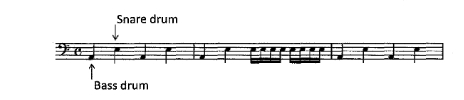
\includegraphics[width=6cm]{Arao_f1.jpg}
  \caption{The phrase with subdivisions of veats used in the experiment\cite{Arao}.}
  \label{Arao_f1}
\end{figure}
\begin{figure}
  \centering
  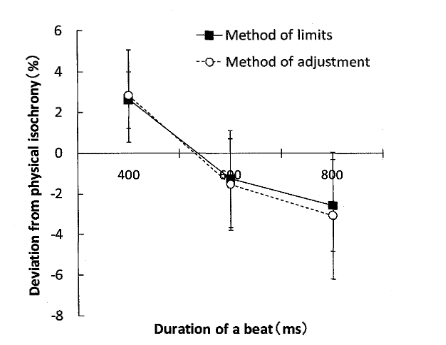
\includegraphics[width=6cm]{Arao_f2.jpg}
  \caption{Deviation from physical isochrony as a function og the duration of a beat in the ecperiment using phrases with subdivisions.Eroor bars represent 95\% confidence intervals\cite{Arao}.}
  \label{Arao_f2}
\end{figure}
\begin{figure}
  \centering
  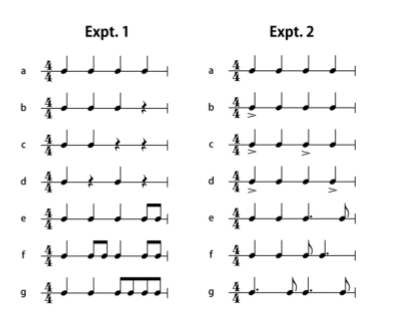
\includegraphics[width=6cm]{Nagasima.jpg}
  \caption{実験で用いたリズムパタン\cite{Nagasima}.}
  \label{Nagasima}
\end{figure}
\begin{figure}
  \centering
  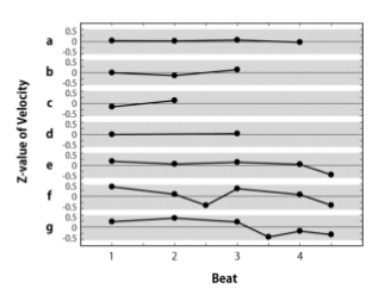
\includegraphics[width=6cm]{Nagasima_2.jpg}
  \caption{打鍵速度のリズムパタン依存性\cite{Nagasima}.}
  \label{Nagasima}
\end{figure}

\section{実験方法}
\subsection{被験者}
本実験には10名(男性○、女性○)の被験者が参加した。楽器演奏経験の乏しい被験者では安定したリズムパタンの再生が困難である場合が多いため、本実験の被験者には何らかの楽器演奏経験がある被験者のみを対象に行った。被験者には謝礼として、図書カード1000円分を手渡した。

\subsection{課題}
本実験には、従来の研究と同様に同期・継続課題を用いる。本実験では、同期区間を32拍分(4分の4拍子で8小節)、継続区間を拍分240(4分の4拍子で60小節)とした。

本研究では、Collyerの報告 \cite{Collyer}においてテンポ変化が生じにくかった120 bpmを目標テンポに設定して目標リズム音を作成した。

\subsection{装置}
被験者のタッピング動作の記録には、Arduinoに圧力センサ、赤外線距離センサを組み合わせたスイッチを用いる。被験者はこのスイッチを人差し指でタッピングすることにより課題を遂行する。Arduino上でUSBケーブルを介してシリアル通信をデータ転送レート9600 bpsで行い、計測PC上でProcessingにて作成したプログラムに随時転送し、テキストファイルとして出力した。時間はサンプリング周波数から割り出した値を後から追加した。同期時の基準テンポとしてはメトロノーム音源をmp3形式のファイルとして作成し、Arduino DFPlayerにて計測開始から24拍(4分の4拍子で8小節)のみ再生した。再生にはスピーカー(なんかのやつ)を使用し、被験者ごとに快適な音量に調節した。

測定時、被験者には椅子に座り、机上のスイッチをタッピングするように指示した。タッピングをする際に使用する腕は、被験者に左右どちらがタッピングを行いやすいか確認をとり、被験者が選んだ腕でタッピングを行ってもらった。なお、被験者には腕の疲労が溜まりにくいように、高さ7 cmのクッションを机上に設置し、肘から手首にかけてクッションにおいてもらい、手首を振り下ろす形でタッピングを行ってもらった。

\subsection{条件}
本実験では、タッピング間隔が一定である統制条件と、他合計8種類のリズムおよびアクセントパタンでタッピングを行う条件を設けた。条件aは統制条件、c-dは(2.永島 亮誠, 阪口 豊)の研究で加速が見られたパタン、e-fは同実験で減速が見られたパタン、g-hは2小節を1つとしたリズムパタンである。

\subsection{手続き}
実験で使用するリズムに慣れるために、各リズムを使用した実験を行う前に、そのリズムで同期区間8小節、継続区間8小節の練習課題を課した。被験者がリズムパタンを理解し、タッピングできることを確認した後、同期区間 32拍分、継続区間 320拍分の本試験を行った。1試行に要した時間は2分弱である。したがって、実験全体で要した時間は、準備の時間も含めておよそ1時間だった。
\begin{center}
	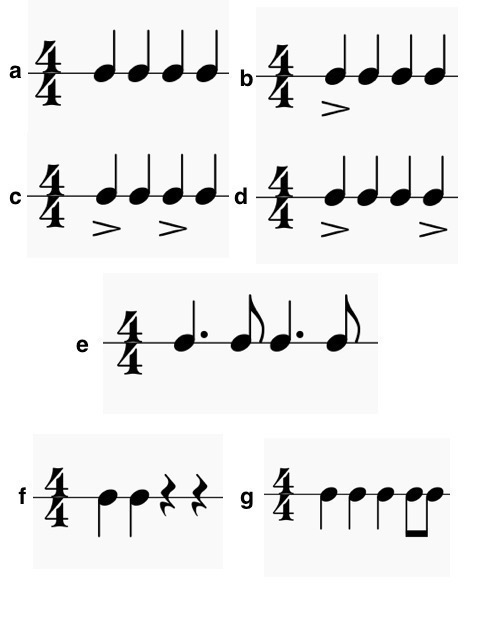
\includegraphics[width=3cm]{patna_g.jpeg}
\end{center}	
\begin{center}
	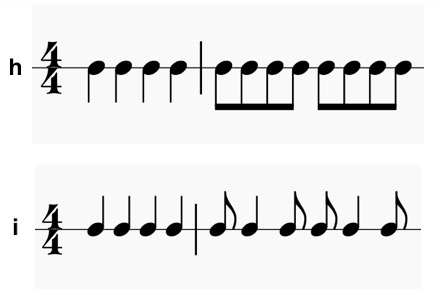
\includegraphics[width=3cm]{patnh_i.jpeg}
\end{center}	

\subsection{解析}
本実験の結果を統計的に検証するため、第2から第80までの各小節の小節長と第1小節の小節長との違いを順序尺度により検定した。

\bibliography{design}
\bibliographystyle{junsrt}

\end{document}
